\documentclass{article}
\usepackage[margin=1.0in]{geometry}
\usepackage{amsmath, amssymb, mathrsfs}
\usepackage[english]{babel}
\usepackage{graphicx}
\usepackage{enumerate}
\usepackage{tikz}
\usetikzlibrary{shapes,backgrounds}

\title{Numerical Computing HW 5}
\author{Greg Stewart}
\date{\today}

\begin{document}

\maketitle

\section*{6.1 (d), (e)}

\begin{enumerate}[(a)]\setcounter{enumi}{4}
  \item \textit{Using the composite trapezoirdal rule, how small does the step size $h$ have to be to guarantee that the numerical error is less than $10^{-6}$?}

    To find $h$, we set the error formula to $10^{-6}$ and solve.

    \begin{align*}
      -\frac{1}{12}h^3f''(\eta) &= 10^{-6} \\
      h^3 &= \frac{12 \times 10^{-6}}{f''(\eta)} \\
      h &= \Big[\frac{12 \times 10^{-6}}{f''(\eta)}\Big]^{1/3} 
    \end{align*}

    Taking $f(x) = x^2$, this means we have $h$

    $$h = 0.01817...$$
  \item \textit{Using the composite Simpson's rule, how small does the step size $h$ have to be to guarantee that the numerical eroor is less than $10^{-6}$?}

    We solve this the same way.

    \begin{align*}
      -\frac{1}{90}h^5f''''(\eta) &= 10^{-6} \\
      h^5 &= \frac{90 \times 10^{-6}}{f''''(\eta)} \\
      h &= \Big[\frac{90 \times 10^{-6}}{f''''(\eta)}\Big]^{1/5}
    \end{align*}

    Takign $f(x) = x^4$, we get for $h$

    $$h = 0.08219...$$ 
\end{enumerate}


\section*{6.4 (a)---(d)}

\textit{For a linearly elastic material, the stress is given by}

$$T = E \frac{du}{dx}$$

\noindent\textit{where $u(x)$ is the displacement of the material and $E$ is a positive constant known as the Young's modulus. The question considered here is how to determine $u$ from measurements of $T$:}

\begin{table}[h!]
  \centering
  \begin{tabular} {c | c c c c c }
    $x$ & 0 & $\frac{1}{4}$ & $\frac{1}{2}$ & $\frac{3}{4}$ & 1 \\ 
    \hline  
    $T$ & 1 & -1 & 2 & 3 & 4 \\
  \end{tabular}
\end{table}


\begin{enumerate}[(a)]
  \item \textit{Show that}

    $$u(x) = u(0) + \frac{1}{E}\int_0^x T(s)ds$$

    Let's start with some good old fashioned separation of variables:

    \begin{align*}
      du &= \frac{T}{E}dx \\
    \end{align*}

    We can integrate both of these from 0 to $x$ with respect to dummy variables.
    \begin{align*}
      \int_0^x du &= \frac{1}{E} \int_0^x T(s)ds \\
      u(x) - u(0) &= \frac{1}{E} \int_0^x T(s)ds \\
      u(x) &= u(0) + \frac{1}{E} \int_0^x T(s)ds
    \end{align*}

    And this final equation is what we wanted.

    Note that for the following parts $u(0) = 0$ and $E = 4$.
  \item \textit{Use the trapezoidal rule to find the value of $u(x)$ at each nonzero x value.}

    The trapezoidal rule is 

    $$\int_{x_i}^{x_{i+1}} f(x)dx \approx \frac{h}{2}(f_i + f_{i+1})$$

    We take $x_i$ on the LHS to be 0 in this case, and evaluate the RHS of the expression from (a) using this rule.

    \begin{table}[h!]
      \centering
      \def\arraystretch{1.5}
      \begin{tabular}{c | c}
        $x$ & $u(x)$ \\
        \hline
        $\frac{1}{4}$ & $\frac{1}{4} (\frac{1}{8}(1 + (-1))) = 0$ \\
        $\frac{1}{2}$ & $u(1/4) + \frac{1}{4}(\frac{1}{8}(-1 + 2)) = \frac{1}{32}$ \\
        $\frac{3}{4}$ & $u(1/2) + \frac{1}{4}(\frac{1}{8}(2 + 3)) = \frac{3}{16}$ \\
        1 & $u(3/4) + \frac{1}{4}\frac{1}{8}(3+4) = \frac{13}{32}$
      \end{tabular}
    \end{table}
  \item \textit{Use the composite midpoint rule to calculate $u(1)$.}

    Since we have no continuous function to evaluate, we can only use two midpoints from the data to evaluate the integral. So we have

    \begin{align*}
      u(1) &= \frac{1}{4} (\frac{1}{2}\cdot (-1) + \frac{1}{2}\cdot 3) \\
      u(1) &= \frac{1}{4}
    \end{align*}
  \item \textit{Use the composite Simpson rule to do the same thing.}
    
    We can be a bit more precise here, and take $h=\frac{1}{4}$.

    \begin{align*}
      u(1) &= \frac{1}{4}\Big[\frac{1/4}{3}(1 + 4(-1) + 2) + \frac{1/4}{3}(-1 + 4(2) + 3) + \frac{1/4}{3}(2 + 12 + 4)\Big] \\
      u(1) &= \frac{1}{4}\Big[\frac{1}{12} (-1) + \frac{1}{12} (10) + \frac{1}{12} (18)\Big] \\
      u(1) &= \frac{1}{4}\Big[\frac{9}{4}\Big] \\
      u(1) &= \frac{9}{16}
    \end{align*}
\end{enumerate}


\section*{6.15 (a), (c)}

\textit{}

\begin{enumerate}[(a)]
  \item \textit{Given subinterval $t_i \leq t \leq t_{i+1}$, then $a_i$ and $a_{i+1}$ are known. Assuming $v_i$ and $y_i$ habe already been computed, use the trapezoidal rule to obtain the following expressions:}
    \begin{align}
      v_{i+1} &= v_i + \frac{1}{2}h(a_i + a_{i+1}) \\
      y_{i+1} &= y_i + \frac{1}{2}h(v_i + v_{i+1}) 
    \end{align}

    The trapezoidal rule is given by 

    $$\int_{x_i}^{x_{i+1}} f(x)dx \approx \frac{h}{2} (f_{i+1} + f_i)$$

    So replacing $f(x)$ with $a(t)$, we get 

    $$\int_{t_i}^{t_{i+1}} a(t)dt \approx \frac{h}{2} (a_{i+1} + a_i)$$

    Of course, integrating $a(t)$ gives us the change in velocity over this interval:

    $$\Delta v = v_{i+1} - v_i = \frac{h}{2} (a_{i+1} + a_i)$$

    Which can just be rewritten as

    $$v_{i+1} = v_i + \frac{h}{2} (a_{i+1} + a_i)$$

    And this matches what we wanted for (1). (2) is obtained in exactly the same way, except that $v(t)$ is integrated.
    
    $$\int_{t_i}^{t_{i+1}} v(t)dt \approx \frac{h}{2} (v_{i+1} + v_i)$$

    And we use the fact that position is given by the integral of velocity to write

    $$y_{i+1} = y_i + \frac{h}{2} (v_{i+1} + v_i)$$

    Which is what we wanted for (2).

\end{enumerate}
\begin{enumerate}[(a)]\setcounter{enumi}{2}
  \item \textit{An accurate computed value at $t = 3$ is $y(3) = .72732289075\dots$. What is the difference between this value and what you compute for $y(3)$ at $n = 10, 20, 40$? How large need $n$ be so that the error between the two is less than $10^{-8}$?}
\end{enumerate}

Based on my MATLAB results and checking, $n$ must be about 4000 to achieve an error of less than $10^-8$. 

\bigskip

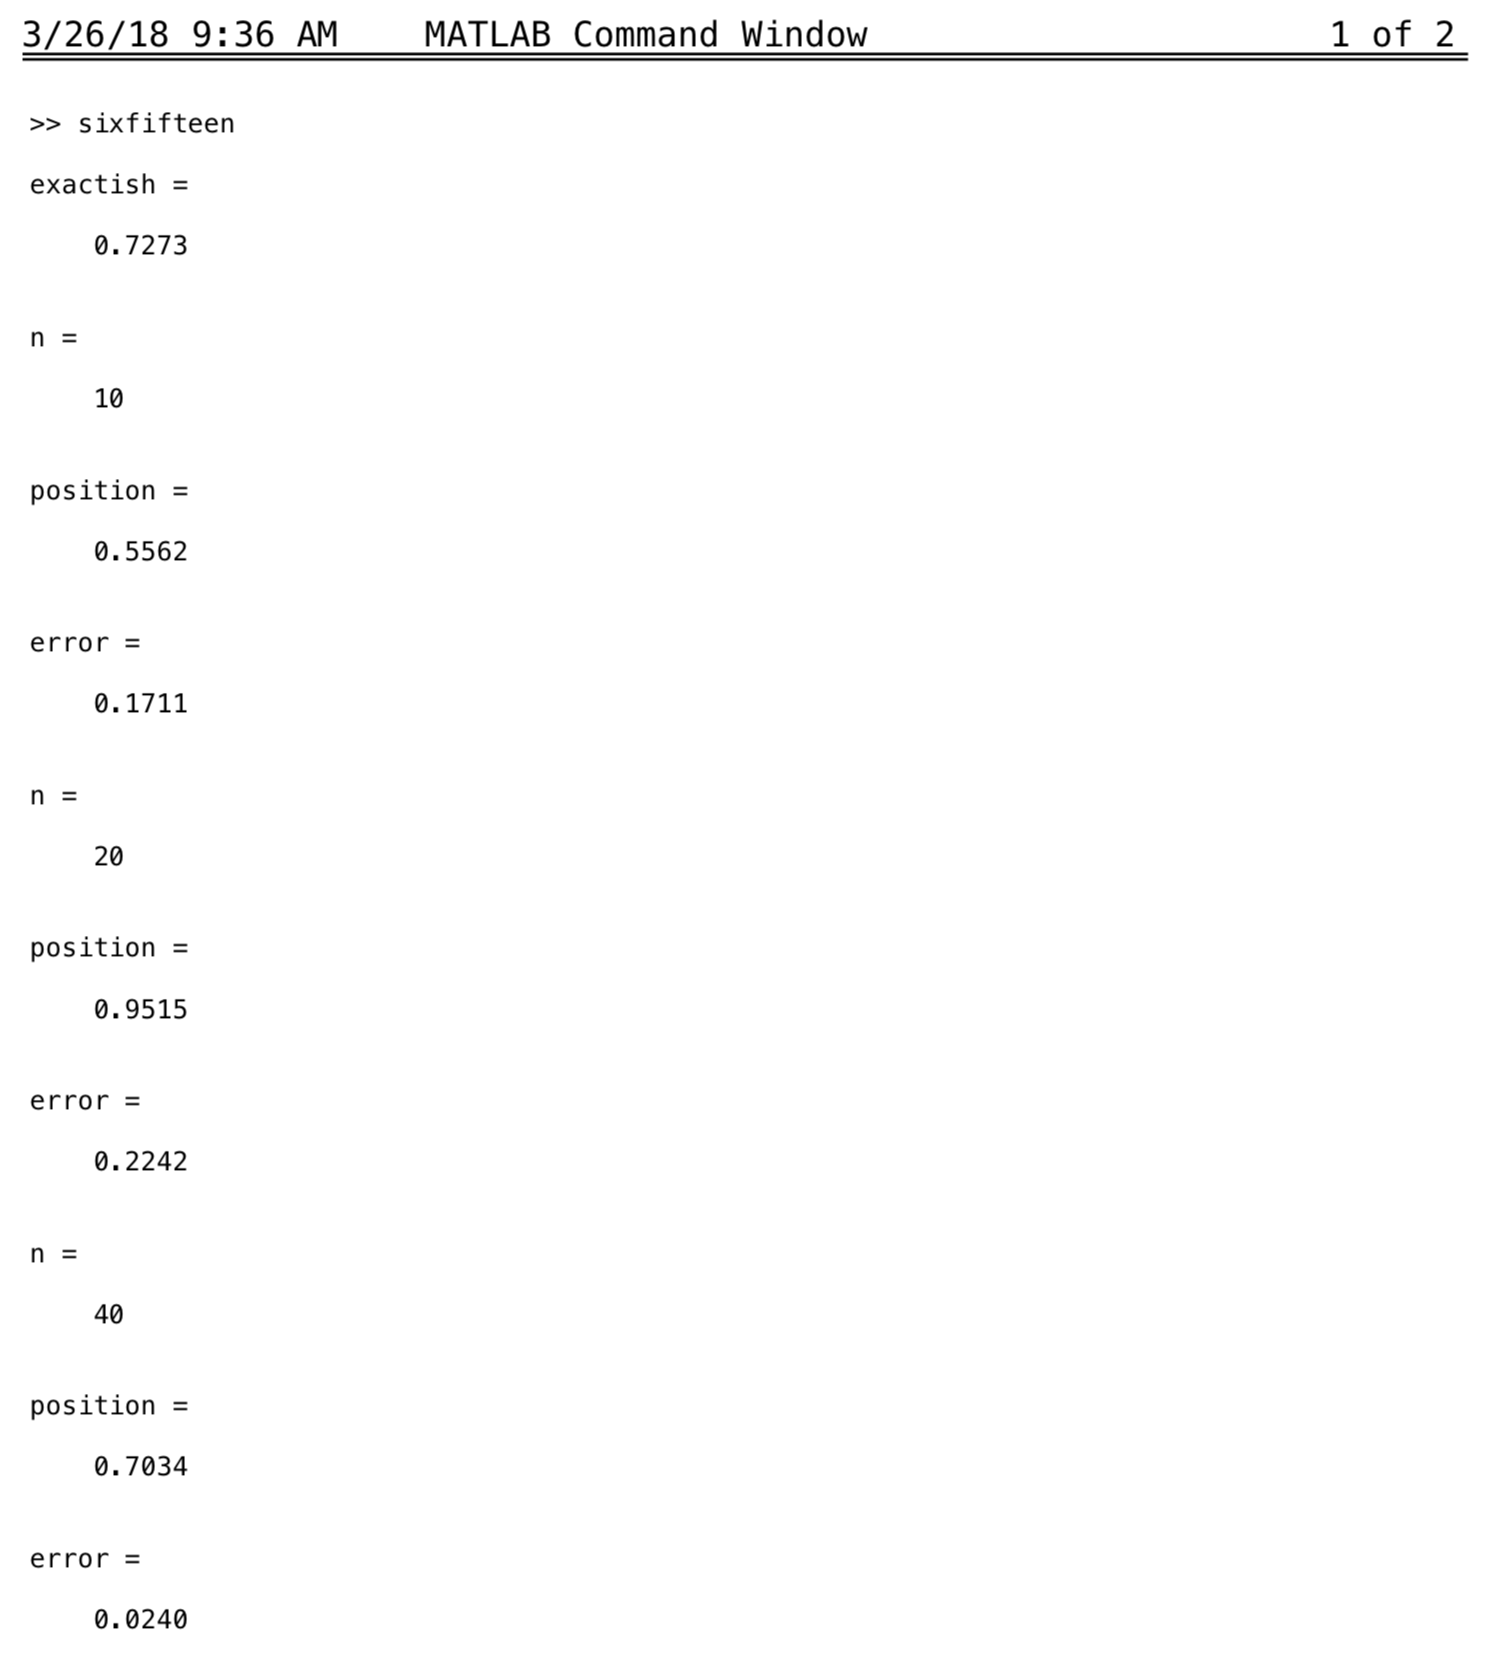
\includegraphics[width=\textwidth]{output.png}
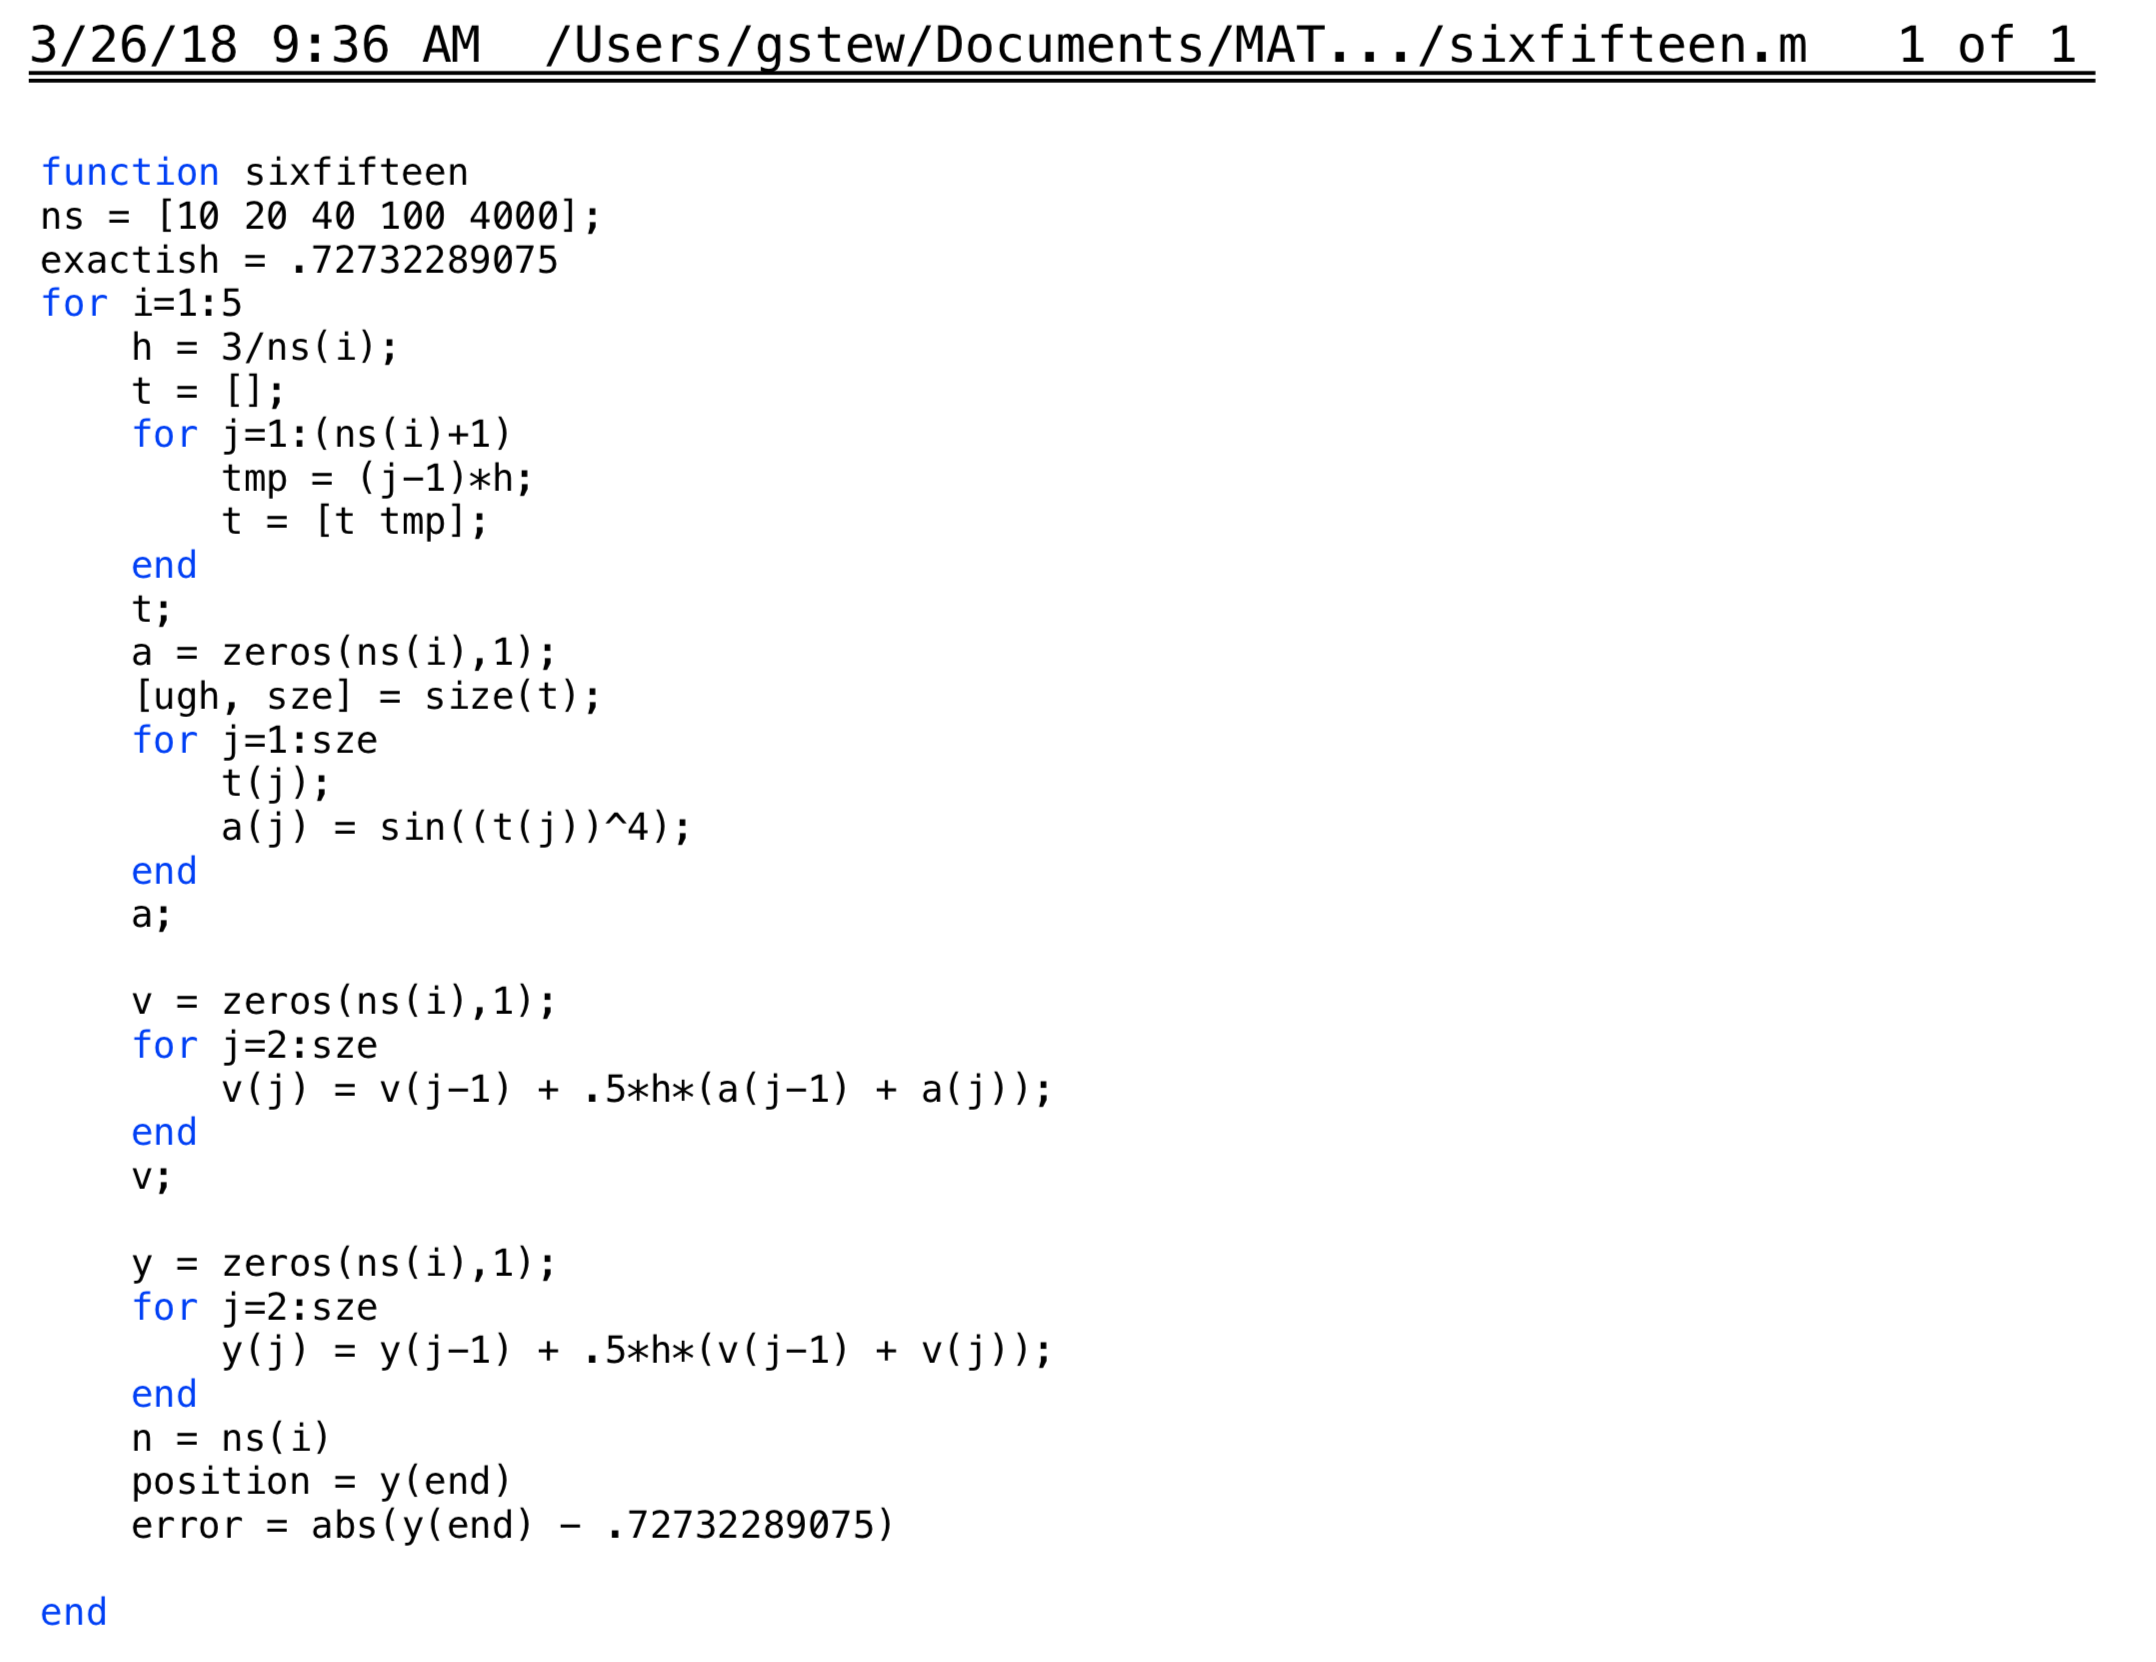
\includegraphics[width=\textwidth]{code.png}

\section*{6.21}

\textit{Suppose the integration rule has form}

$$\int_{x_i}^{x_{i+1}} f(x)dx \approx w_1f(x_i) + w_2f(z)$$

\noindent\textit{This is an example of Radau quadrature, which means that only one of the points used is an endpoint.}

\begin{enumerate}[(a)]
  \item \textit{Find the values of $w_1, w_2, z$ that maximize the precision.}

    To do this we will take $z$ to have the form $z = x_i + \alpha h$ and solve for alpha in addition to the other two unknowns.

    \begin{align*}
      f(x) = 1 \implies &w_1 + w_2 = h \\
      f(x) = x \implies &h(x_i + \frac{h}{2}) = w_1 x_i + w_2 (x_i + \alpha h) \\
      &h(x_i+\frac{h}{2}) = (w_1 + w_2)x_i + w_2 \alpha h \\
      &h(x_i+\frac{h}{2}) = h x_i + w_2 \alpha h \\
      &\frac{h}{2} = w_2 \alpha h \\
      &\alpha = \frac{h}{2w_2} \\
      f(x) = x^2 \implies &h(x_i^2 + hx_i + \frac{1}{3}h^2) = w_1x_i^2 + w_2(x_i^2 + 2x_i\alpha h+ \alpha^2h^2) \\
      &h(x_i^2 + hx_i + \frac{1}{3}h^2) = (w_1 + w_2)x_i^2 + w_2\frac{x_i h^2}{w_2}+ w_2\frac{h^4}{4w_2^2} \\
      &\frac{1}{3}h^3 = \frac{h^4}{4w_2} \\
      &w_2 = \frac{3h}{4} \\
      &\implies w_1 + \frac{3h}{4} = h \\
      &\implies w_1 = \frac{h}{4} \\
      &\implies \alpha = \frac{4h}{6h} = \frac{2}{3}
    \end{align*}
  \item \textit{The error is know to have form}

    $$\int_{x_i}^{x_{i+1}}f(x)dx = w_1f(x_i) + w_2 f(z) + K h^4 f'''(\eta)$$

    \textit{where, as usual, $\eta$ is a point somewhere in the interval. Find $K$.}

    We solve for $K$ by taking $f(x) = x^3$, which means that $f'''(\eta) = 6$. Thus we have

    \begin{align*}
      h(x_i^3 + \frac{3hx_i^2}{2} + h^2 x_i + \frac{h^3}{4}) &= \frac{h}{4}x_i^3 + \frac{3h}{4}(x_i + \frac{2h}{3})^3 + 6h^4K \\
      &= \frac{hx_i^3}{4} + \frac{3h}{4}(x_i^3 + 3\cdot\frac{2hx_i^2}{3} + 3\cdot\frac{4h^2x_i}{9} + \frac{8h^3}{27} + 6h^4K \\
      &= hx_i^3 + \frac{3h^2x_i^2}{2} + h^3x_i + \frac{2h^4}{9} + 6h^4K \\
      \frac{h^4}{4} &= \frac{2h^4}{9} + 6h^4K \\
      \frac{1}{36} &= 6K \\
      K &= \frac{1}{216}
    \end{align*}
\end{enumerate}




















\end{document}
